\documentclass[11pt,a4paper]{report}
\usepackage[textwidth=37em,vmargin=30mm]{geometry}
\usepackage{calc,xunicode,amsmath,amssymb,paralist,enumitem,tabu,booktabs,datetime2,xeCJK,xeCJKfntef,listings}
\usepackage{tocloft,fancyhdr,tcolorbox,xcolor,graphicx,eso-pic,xltxtra,xelatexemoji}

\newcommand{\envyear}[0]{2025}
\newcommand{\envdatestr}[0]{2025-07-25}
\newcommand{\envfinaldir}[0]{webdb/2025/20250725/final}

\usepackage[hidelinks]{hyperref}
\hypersetup{
    colorlinks=false,
    pdfpagemode=FullScreen,
    pdftitle={Web Digest - \envdatestr}
}

\setlength{\cftbeforechapskip}{10pt}
\renewcommand{\cftchapfont}{\rmfamily\bfseries\large\raggedright}
\setlength{\cftbeforesecskip}{2pt}
\renewcommand{\cftsecfont}{\sffamily\small\raggedright}

\setdefaultleftmargin{2em}{2em}{1em}{1em}{1em}{1em}

\usepackage{xeCJK,xeCJKfntef}
\xeCJKsetup{PunctStyle=plain,RubberPunctSkip=false,CJKglue=\strut\hskip 0pt plus 0.1em minus 0.05em,CJKecglue=\strut\hskip 0.22em plus 0.2em}
\XeTeXlinebreaklocale "zh"
\XeTeXlinebreakskip = 0pt


\setmainfont{Brygada 1918}
\setromanfont{Brygada 1918}
\setsansfont{IBM Plex Sans}
\setmonofont{JetBrains Mono NL}
\setCJKmainfont{Noto Serif CJK SC}
\setCJKromanfont{Noto Serif CJK SC}
\setCJKsansfont{Noto Sans CJK SC}
\setCJKmonofont{Noto Sans CJK SC}

\setlength{\parindent}{0pt}
\setlength{\parskip}{8pt}
\linespread{1.15}

\lstset{
	basicstyle=\ttfamily\footnotesize,
	numbersep=5pt,
	backgroundcolor=\color{black!5},
	showspaces=false,
	showstringspaces=false,
	showtabs=false,
	tabsize=2,
	captionpos=b,
	breaklines=true,
	breakatwhitespace=true,
	breakautoindent=true,
	linewidth=\textwidth
}






\newcommand{\coverpic}[2]{
    % argv: itemurl, authorname
    Cover photo by #2~~(\href{#1}{#1})
}
\newcommand{\makeheader}[0]{
    \begin{titlepage}
        % \newgeometry{hmargin=15mm,tmargin=21mm,bmargin=12mm}
        \begin{center}
            
            \rmfamily\scshape
            \fontspec{BaskervilleF}
            \fontspec{Old Standard}
            \fontsize{59pt}{70pt}\selectfont
            WEB\hfill DIGEST
            
            \vfill
            % \vskip 30pt
            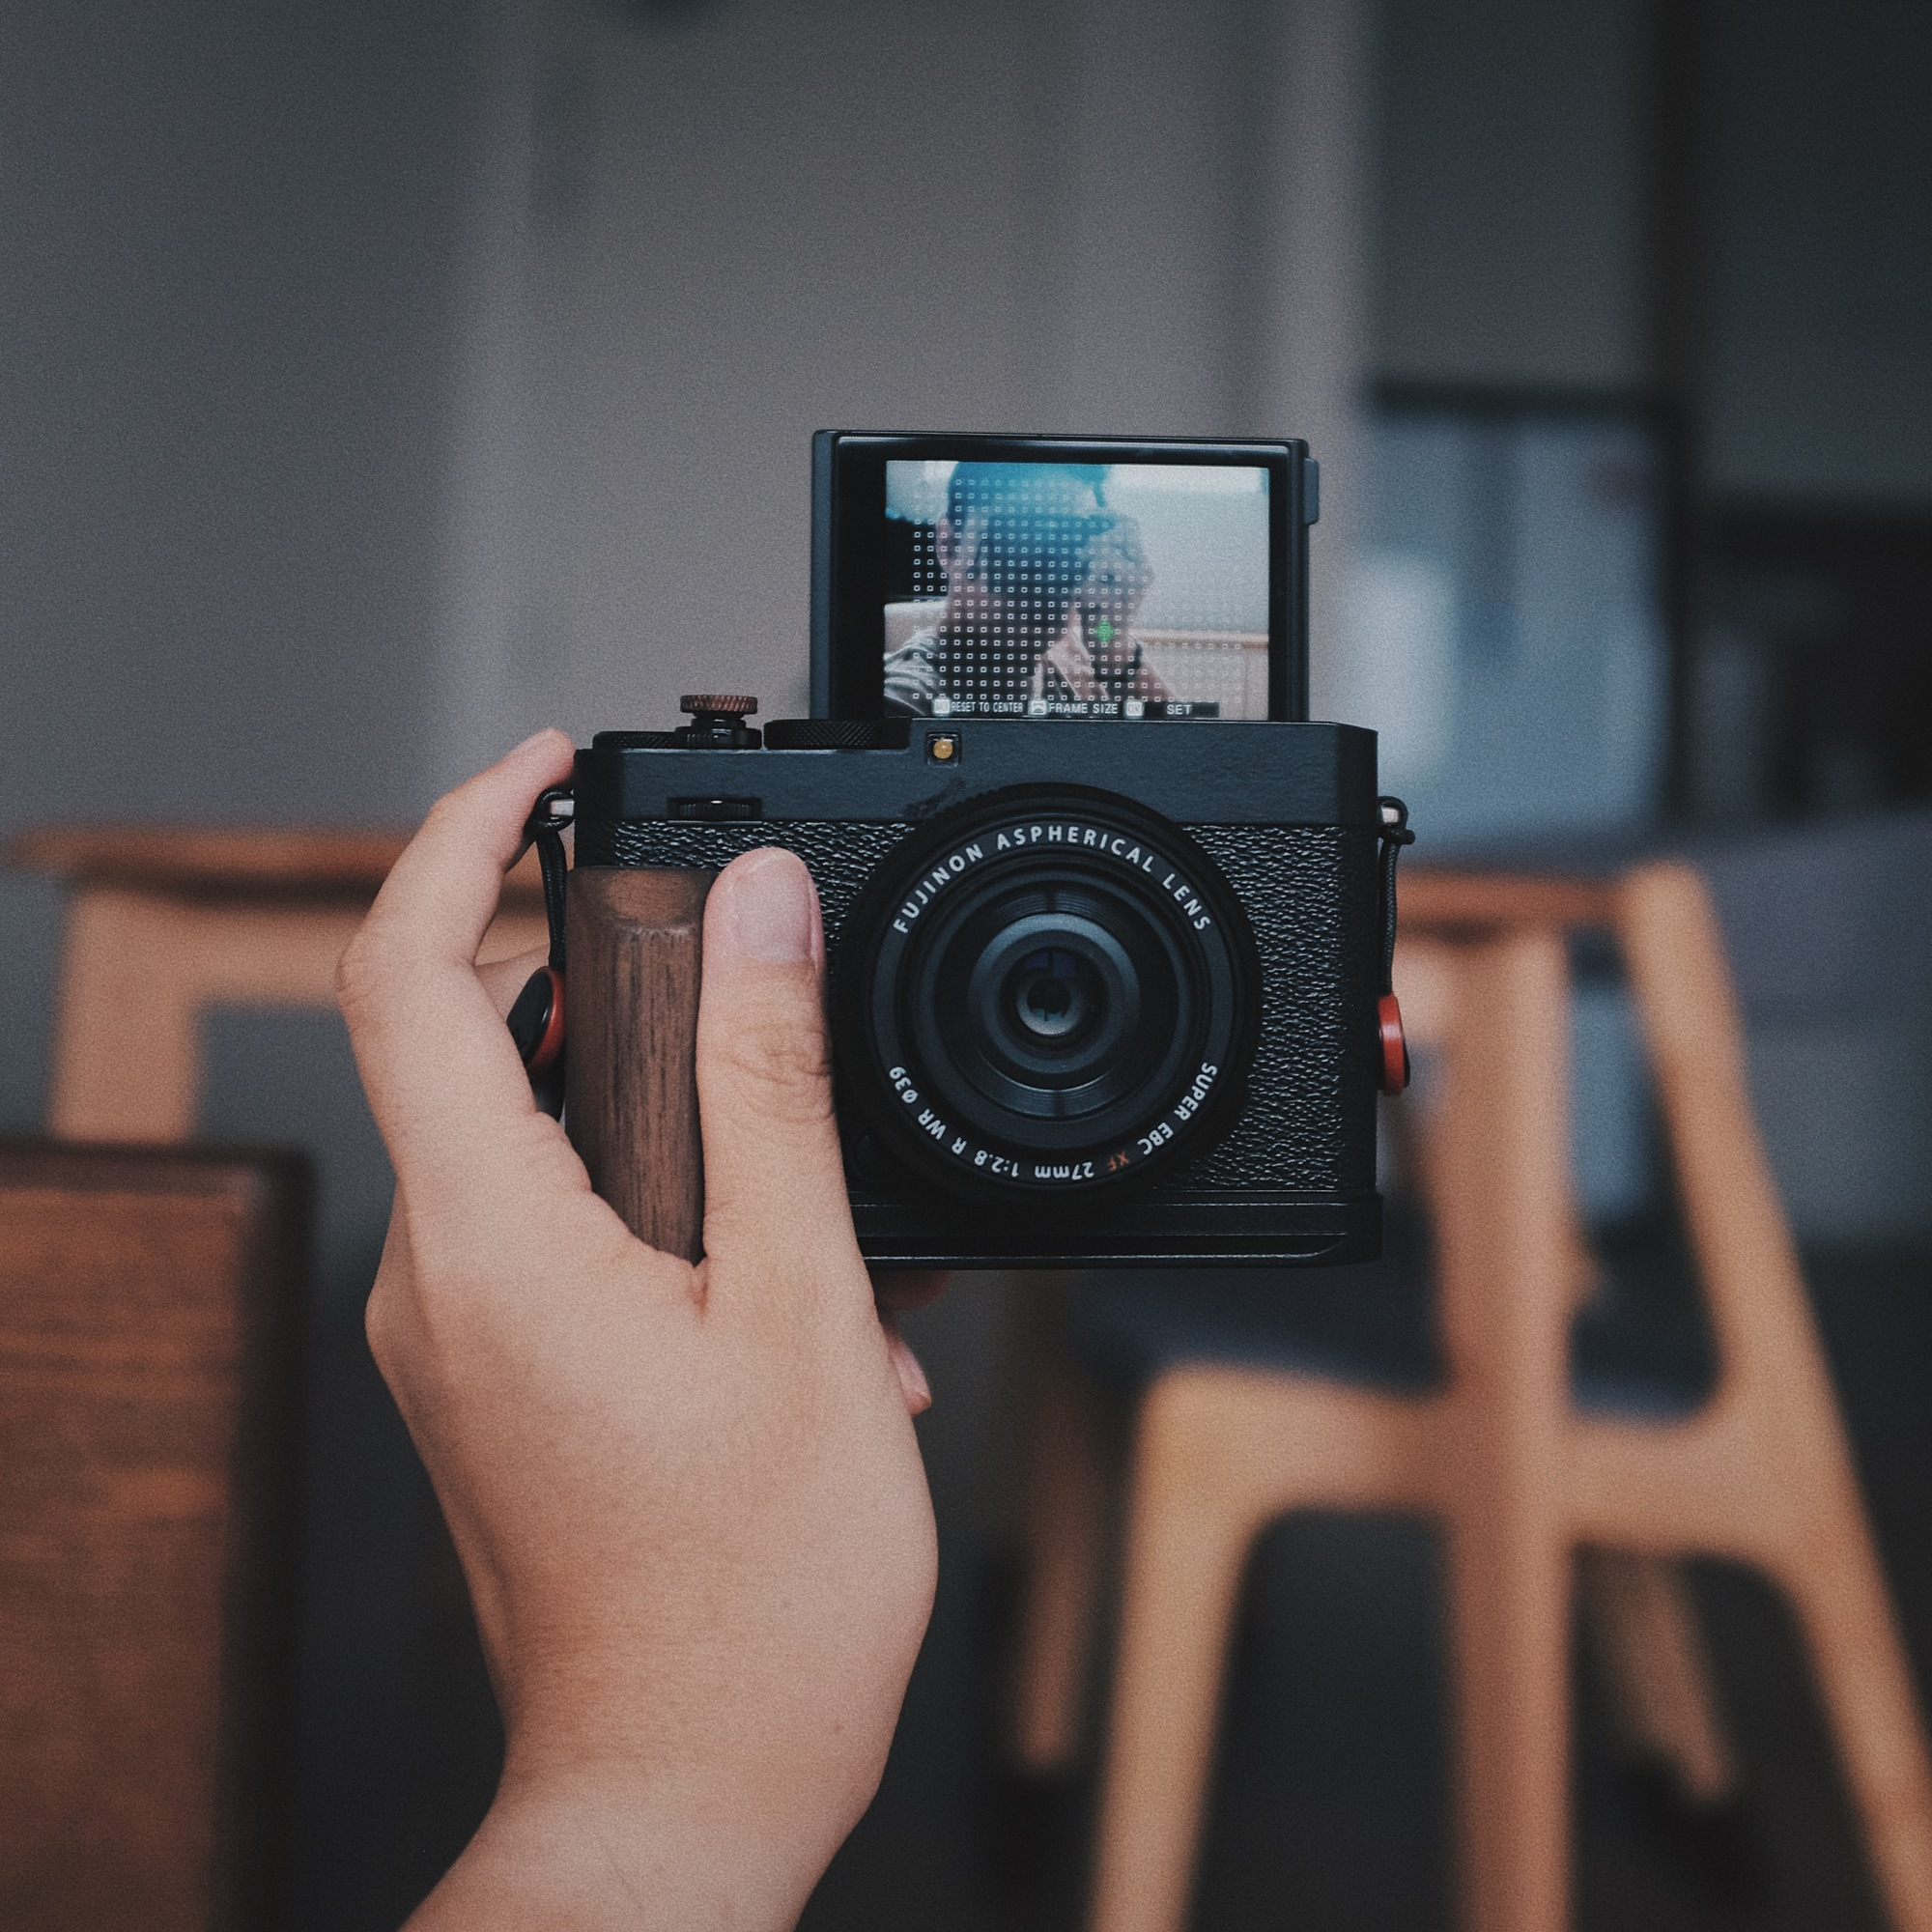
\includegraphics[width=\linewidth]{\envfinaldir/coverpic-prod.jpg}\par
            % \vskip 30pt
            \vfill

            \normalsize\rmfamily\scshape
            \copyright{} The Web Digest Project \hfill\large \envdatestr
        \end{center}
    \end{titlepage}
    % \restoregeometry
}
\newcommand{\simplehref}[1]{%
    \textcolor{blue!80!green}{\href{#1}{#1}}%
}
\renewcommand{\contentsname}{\center\Huge\sffamily\bfseries Contents\par\vskip 20pt}
\newcounter{ipartcounter}
\setcounter{ipartcounter}{0}
\newcommand{\ipart}[1]{
    % \vskip 20pt
    \clearpage
    \stepcounter{ipartcounter}
    \phantomsection
    \addcontentsline{toc}{chapter}{#1}
    % \begin{center}
    %     \Huge
    %     \sffamily\bfseries
    %     #1
    % \end{center}
    % \vskip 20pt plus 7pt
}
\newcounter{ichaptercounter}
\setcounter{ichaptercounter}{0}
\newcommand{\ichapter}[1]{
    % \vskip 20pt
    \clearpage
    \stepcounter{ichaptercounter}
    \phantomsection
    \addcontentsline{toc}{section}{\numberline{\arabic{ichaptercounter}}#1}
    \begin{center}
        \Huge
        \sffamily\bfseries
        #1
    \end{center}
    \vskip 20pt plus 7pt
}
\newcommand{\entrytitlefont}[1]{\subsection*{\raggedright\Large\sffamily\bfseries#1}}
\newcommand{\entryitemGeneric}[2]{
    % argv: title, url
    \parbox{\linewidth}{
        \entrytitlefont{#1}\par\vskip 5pt
        \footnotesize\ttfamily\mdseries
        \simplehref{#2}
    }\vskip 11pt plus 11pt minus 1pt
}
\newcommand{\entryitemGithub}[3]{
    % argv: title, url, desc
    \parbox{\linewidth}{
        \entrytitlefont{#1}\par\vskip 5pt
        \footnotesize\ttfamily\mdseries
        \simplehref{#2}\par\vskip 5pt
        \small\rmfamily\mdseries#3
    }\vskip 11pt plus 11pt minus 1pt
}
\newcommand{\entryitemAp}[3]{
    % argv: title, url, desc
    \parbox{\linewidth}{
        \entrytitlefont{#1}\par\vskip 5pt
        \footnotesize\ttfamily\mdseries
        \simplehref{#2}\par\vskip 5pt
        \small\rmfamily\mdseries#3
    }\vskip 11pt plus 11pt minus 1pt
}
\newcommand{\entryitemHackernews}[3]{
    % argv: title, hnurl, rawurl
    % \parbox{\linewidth}{
    %     \entrytitlefont{#1}\par\vskip 5pt
    %     \footnotesize\ttfamily\mdseries
    %     \simplehref{#3}\par
    %     \textcolor{black!50}{\href{#2}{#2}}
    % }\vskip 11pt plus 11pt minus 1pt
    \begin{minipage}{\linewidth}
            \entrytitlefont{#1}\par\vskip 5pt
            \footnotesize\ttfamily\mdseries
            \simplehref{#3}\par
            \textcolor{black!50}{\href{#2}{#2}}
    \end{minipage}\par\vskip 11pt plus 11pt minus 1pt
}







\begin{document}

\makeheader

\tableofcontents\clearpage




\ipart{Developers}
\ichapter{Hacker News}
\entryitemTwoLinks{Visa and Mastercard: The global payment duopoly (2024)}{https://news.ycombinator.com/item?id=44676559}{https://quartr.com/insights/edge/visa-and-mastercard-the-global-payment-duopoly}

\entryitemTwoLinks{Intel CEO Letter to Employees}{https://news.ycombinator.com/item?id=44675965}{https://morethanmoore.substack.com/p/intel-ceo-letter-to-employees}

\entryitemTwoLinks{Starlink is currently experiencing a service outage}{https://news.ycombinator.com/item?id=44674960}{https://www.starlink.com/us}

\entryitemTwoLinks{Major quantum computing advance made obsolete by teenager (2018)}{https://news.ycombinator.com/item?id=44672859}{https://www.quantamagazine.org/teenager-finds-classical-alternative-to-quantum-recommendation-algorithm-20180731/}

\entryitemTwoLinks{Two narratives about AI}{https://news.ycombinator.com/item?id=44672414}{https://calnewport.com/no-one-knows-anything-about-ai/}

\entryitemTwoLinks{There is no memory safety without thread safety}{https://news.ycombinator.com/item?id=44672003}{https://www.ralfj.de/blog/2025/07/24/memory-safety.html}

\entryitemTwoLinks{Use Your Type System}{https://news.ycombinator.com/item?id=44671484}{https://www.dzombak.com/blog/2025/07/use-your-type-system/}

\entryitemTwoLinks{A list of changes to make it easier to build beautiful and walkable places}{https://news.ycombinator.com/item?id=44671472}{https://chrisbarber.co/A+list+of+changes+to+make+it+easier+to+build+beautiful+\%26+walkable+places}

\entryitemTwoLinks{PSA: SQLite WAL checksums fail silently and may lose data}{https://news.ycombinator.com/item?id=44671373}{https://avi.im/blag/2025/sqlite-wal-checksum/}

\entryitemTwoLinks{AMD CEO says U.S.-made TSMC chips are 5\%-20\% more expensive, but worth it}{https://news.ycombinator.com/item?id=44670624}{https://www.tomshardware.com/tech-industry/amd-ceo-says-u-s-made-tsmc-chips-are-more-expensive-but-worth-it-costs-more-than-5-percent-but-less-than-20-percent-higher-than-taiwan-sourced-alternative}

\entryitemTwoLinks{Diet, not lack of exercise, drives obesity, a new study finds}{https://news.ycombinator.com/item?id=44670590}{https://www.npr.org/2025/07/24/nx-s1-5477662/diet-exercise-obesity-nutrition}

\entryitemTwoLinks{UK: Phone networks down: EE, BT, Three, Vodafone, O2 not working in mass outage}{https://news.ycombinator.com/item?id=44670326}{https://www.the-independent.com/tech/ee-bt-three-vodafone-o2-down-phone-networks-outage-latest-b2795260.html}

\entryitemTwoLinks{A valid HTML zip bomb}{https://news.ycombinator.com/item?id=44670319}{https://ache.one/notes/html\_zip\_bomb}

\entryitemTwoLinks{Vet is a safety net for the curl | bash pattern}{https://news.ycombinator.com/item?id=44669998}{https://github.com/vet-run/vet}

\entryitemTwoLinks{Open Source Maintenance Fee}{https://news.ycombinator.com/item?id=44669858}{https://github.com/wixtoolset/issues/issues/8974}

\entryitemTwoLinks{Web fingerprinting is worse than I thought (2023)}{https://news.ycombinator.com/item?id=44669853}{https://www.bitestring.com/posts/2023-03-19-web-fingerprinting-is-worse-than-I-thought.html}

\entryitemTwoLinks{Itch.io: Update on NSFW Content}{https://news.ycombinator.com/item?id=44667667}{https://itch.io/updates/update-on-nsfw-content}

\entryitemTwoLinks{Apache HTTP Server: 'RewriteCond expr' always evaluates to true}{https://news.ycombinator.com/item?id=44666896}{https://github.com/apache/httpd/commit/8abb3d06b23975705ebcf4bf4476464fd0b9bd0b}

\entryitemTwoLinks{Electric cars produce less brake dust pollution than combustion-engine cars}{https://news.ycombinator.com/item?id=44666157}{https://modernengineeringmarvels.com/2025/07/22/surprising-science-how-electric-cars-quietly-transform-urban-air/}

\entryitemTwoLinks{A small web July}{https://news.ycombinator.com/item?id=44665984}{https://smallcypress.bearblog.dev/a-small-web-july/}


\ipart{Developers~~~~(zh-Hans)}
\ichapter{Solidot}
\entryitemGeneric{\hskip 0pt{}FDA 的 AI 工具被发现捏造研究}{https://www.solidot.org/story?sid=81881}

\entryitemGeneric{\hskip 0pt{}硅谷 AI 创业公司拥抱中国的 996 工作制}{https://www.solidot.org/story?sid=81880}

\entryitemGeneric{\hskip 0pt{}图瓦卢逾八成国民寻求澳大利亚的气候移民签证}{https://www.solidot.org/story?sid=81879}

\entryitemGeneric{\hskip 0pt{}索尼通过降低 PS5 性能应对全球气候变化}{https://www.solidot.org/story?sid=81877}

\entryitemGeneric{\hskip 0pt{}AWS 关闭上海 AI 研究中心}{https://www.solidot.org/story?sid=81876}

\entryitemGeneric{\hskip 0pt{}英国将禁止公共部门向勒索软件组织支付赎金}{https://www.solidot.org/story?sid=81875}

\entryitemGeneric{\hskip 0pt{}Steam 之后 Itch.io 限制成人游戏}{https://www.solidot.org/story?sid=81874}

\entryitemGeneric{\hskip 0pt{}热浪下欧洲软化对空调的抵制}{https://www.solidot.org/story?sid=81873}

\entryitemGeneric{\hskip 0pt{}气候变化导致森林火灾日益常见}{https://www.solidot.org/story?sid=81872}

\entryitemGeneric{\hskip 0pt{}美国政府考虑重新评估 H-1B 签证签发方式}{https://www.solidot.org/story?sid=81871}

\entryitemGeneric{\hskip 0pt{}ChatGPT 用户每天发送 25 亿提示词}{https://www.solidot.org/story?sid=81870}

\entryitemGeneric{\hskip 0pt{}Brave 浏览器默认屏蔽 Microsoft Recall}{https://www.solidot.org/story?sid=81869}

\entryitemGeneric{\hskip 0pt{}10\%-25\% 的肺癌患者从未吸烟}{https://www.solidot.org/story?sid=81868}

\entryitemGeneric{\hskip 0pt{}研究发现 AI 摘要会显著降低搜索结果页的点击率}{https://www.solidot.org/story?sid=81867}

\entryitemGeneric{\hskip 0pt{}微软从 Google DeepMind 挖走了至少 24 名 AI 工程师}{https://www.solidot.org/story?sid=81866}

\entryitemGeneric{\hskip 0pt{}NASA 如何从 8 亿公里外拯救朱诺号的相机}{https://www.solidot.org/story?sid=81865}

\entryitemGeneric{\hskip 0pt{}法庭裁决 Mike Lynch 的遗产以及商业伙伴欠惠普 9.44 亿美元 }{https://www.solidot.org/story?sid=81864}

\entryitemGeneric{\hskip 0pt{}阿里巴巴发布 Qwen3-Coder}{https://www.solidot.org/story?sid=81863}

\entryitemGeneric{\hskip 0pt{}乐观主义者是相似的但悲观主义者是不同的}{https://www.solidot.org/story?sid=81862}

\entryitemGeneric{\hskip 0pt{}Firefox 141 释出}{https://www.solidot.org/story?sid=81861}\ichapter{V2EX}
\entryitemGeneric{\hskip 0pt{}[日本] 请问有在日本的二手交易群么?}{https://www.v2ex.com/t/1147532}

\entryitemGeneric{\hskip 0pt{}[Android] 它是如何通过非常规手段添加``美团视频''到桌面}{https://www.v2ex.com/t/1147531}

\entryitemGeneric{\hskip 0pt{}[远程工作] [帮朋友转发] Web 前端工程师招聘(全远程、无面试、自由时间、不打卡)}{https://www.v2ex.com/t/1147530}

\entryitemGeneric{\hskip 0pt{}[分享发现] BetterLyrics - 一款专为 Windows 打造的沉浸式流畅歌词显示软件}{https://www.v2ex.com/t/1147529}

\entryitemGeneric{\hskip 0pt{}[分享创造] 一个超简单的板英尺计算器, vibe coding 一小时上线}{https://www.v2ex.com/t/1147528}

\entryitemGeneric{\hskip 0pt{}[macOS] macOS Tahoe Public Beta 发布了}{https://www.v2ex.com/t/1147527}

\entryitemGeneric{\hskip 0pt{}[宽带症候群] 为什么运营商不去约谈 pcdn 平台?}{https://www.v2ex.com/t/1147526}

\entryitemGeneric{\hskip 0pt{}[Apple] Apple Pay 加卡怪事,有些能加,有些不能}{https://www.v2ex.com/t/1147525}

\entryitemGeneric{\hskip 0pt{}[音乐] 哪种方式听音乐的成本最低}{https://www.v2ex.com/t/1147524}

\entryitemGeneric{\hskip 0pt{}[Oracle] 一觉醒来,两个 Oracle 账户登录不进去了}{https://www.v2ex.com/t/1147522}

\entryitemGeneric{\hskip 0pt{}[问与答] Cursor Pro 超额之后继续使用 Used Based 用到 50\$}{https://www.v2ex.com/t/1147521}

\entryitemGeneric{\hskip 0pt{}[云修电脑] WIN10 偶发蓝屏,重装系统后蓝屏频率变高了}{https://www.v2ex.com/t/1147519}

\entryitemGeneric{\hskip 0pt{}[程序员] 求推荐, X(Twitter)的爬虫 API 付费平台(有价值的回答,打赏 SOL)}{https://www.v2ex.com/t/1147518}

\entryitemGeneric{\hskip 0pt{}[NAS] 在群晖上运行 podman,有人试过吗?}{https://www.v2ex.com/t/1147517}

\entryitemGeneric{\hskip 0pt{}[程序员] [GitHub 开源] 不写一行代码最快 1 分钟部署一个交互友好炫酷全自动化管理你的 GitHub Star 项目的网站}{https://www.v2ex.com/t/1147516}

\entryitemGeneric{\hskip 0pt{}[问与答] 想给农村老家安装摄像头,有没有推荐的}{https://www.v2ex.com/t/1147515}

\entryitemGeneric{\hskip 0pt{}[VXNA] 申请收录 www.evan.xin}{https://www.v2ex.com/t/1147514}

\entryitemGeneric{\hskip 0pt{}[V2EX] 话说 v 站有官方客户端么?没有的话有推荐的三方么?}{https://www.v2ex.com/t/1147513}

\entryitemGeneric{\hskip 0pt{}[职场话题] 请教一下各位大佬, 内部转岗的问题.}{https://www.v2ex.com/t/1147512}

\entryitemGeneric{\hskip 0pt{}[问与答] 不想继续做开发,想听下转型后大家的现状}{https://www.v2ex.com/t/1147510}

\entryitemGeneric{\hskip 0pt{}[问与答] 好奇大家买了多少个站长的 v2ex,开始为了注册账号买的,没想到现在已经翻倍了}{https://www.v2ex.com/t/1147508}

\entryitemGeneric{\hskip 0pt{}[分享创造] [一个人独立开发] 两个月撸了个``电表轮换系统'',现在真在用了(Web + App)}{https://www.v2ex.com/t/1147507}

\entryitemGeneric{\hskip 0pt{}[程序员] 各位觉得 Qwen3 Coder 480B 的实际表现怎么样? 可以替代 Claude-4-Sonnet/Opus 作为 Claude Code 的调用模型吗?}{https://www.v2ex.com/t/1147506}

\entryitemGeneric{\hskip 0pt{}[程序员] Flutter 社会分享 Instagram WhatsApp-有哪些可靠方案?}{https://www.v2ex.com/t/1147505}

\entryitemGeneric{\hskip 0pt{}[加密货币] 有需要对敲 usdt 或者 usdc 的吗?}{https://www.v2ex.com/t/1147504}

\entryitemGeneric{\hskip 0pt{}[程序员] 关于 Trae 自定义 Gemini 时一直转圈无法正常设置的问题}{https://www.v2ex.com/t/1147503}

\entryitemGeneric{\hskip 0pt{}[iOS] IOS 端跑 webrtc 有 BUG. 熟悉这一块的联系我}{https://www.v2ex.com/t/1147502}

\entryitemGeneric{\hskip 0pt{}[程序员] Python 爬虫入门: 10 分钟抓取豆瓣读书标题}{https://www.v2ex.com/t/1147500}

\entryitemGeneric{\hskip 0pt{}[问与答] mac 端有无免费正常显示 hdr 的 emby 播放器}{https://www.v2ex.com/t/1147499}

\entryitemGeneric{\hskip 0pt{}[分享发现] 用 Claude AI 从零开发了一个完整的 Coldplay 主题游戏 - 全程技术分享}{https://www.v2ex.com/t/1147497}

\entryitemGeneric{\hskip 0pt{}[Solana] 关于部分用户在初次使用打赏功能时在 Phantom 里看到的红框提示}{https://www.v2ex.com/t/1147496}

\entryitemGeneric{\hskip 0pt{}[问与答] MX Master 3S 需要搭配腕托使用吗?}{https://www.v2ex.com/t/1147495}

\entryitemGeneric{\hskip 0pt{}[V2EX] 「空投」抽 20 人送 0.001 SOL -- 明牌赚铜币}{https://www.v2ex.com/t/1147494}

\entryitemGeneric{\hskip 0pt{}[问与答] app 开屏广告为啥爱用陀螺仪跳转呢?}{https://www.v2ex.com/t/1147493}

\entryitemGeneric{\hskip 0pt{}[问与答] 狗爹(GoDaddy)作为域名注册商,自己也炒域名,有点难绷}{https://www.v2ex.com/t/1147492}

\entryitemGeneric{\hskip 0pt{}[问与答] vscode Python 插件自动激活环境配置求助}{https://www.v2ex.com/t/1147491}

\entryitemGeneric{\hskip 0pt{}[数据库] SQL 数据库咨询}{https://www.v2ex.com/t/1147490}

\entryitemGeneric{\hskip 0pt{}[浏览器] 网页浏览器新型狗皮膏药}{https://www.v2ex.com/t/1147488}

\entryitemGeneric{\hskip 0pt{}[问与答] 去年一整年在山姆消费 14000,有必要买卓越卡吗?}{https://www.v2ex.com/t/1147487}

\entryitemGeneric{\hskip 0pt{}[酷工作] 北京:大模型算法研究员-在 AI for Science 领域有实际项目经验}{https://www.v2ex.com/t/1147485}

\entryitemGeneric{\hskip 0pt{}[问与答] 我记得之前有个模糊个人信息的选项,找不到了.有人知道在哪吗.}{https://www.v2ex.com/t/1147484}

\entryitemGeneric{\hskip 0pt{}[问与答] 淘宝或者京东 DIY 装机有用过国补的么?}{https://www.v2ex.com/t/1147483}

\entryitemGeneric{\hskip 0pt{}[问与答] 请大佬检阅,给点意见.}{https://www.v2ex.com/t/1147482}

\entryitemGeneric{\hskip 0pt{}[VXNA] 申请收录个人博客: www.haomwei.com}{https://www.v2ex.com/t/1147481}

\entryitemGeneric{\hskip 0pt{}[酷工作] [急招] 字节跳动 Pico UI Android/高级 Android 开发工程师}{https://www.v2ex.com/t/1147480}

\entryitemGeneric{\hskip 0pt{}[V2EX] 今天终于注册成功 V2EX,记录一下}{https://www.v2ex.com/t/1147479}

\entryitemGeneric{\hskip 0pt{}[求职] [求职上海] IOS 开发, 24 届 1 年经验做过上海地铁项目}{https://www.v2ex.com/t/1147478}

\entryitemGeneric{\hskip 0pt{}[问与答] 兄弟们, AI 可以干掉大部份程序员没有争议, AI 能不能干掉大部份的 ERP 或 CRM 从业人员呢?}{https://www.v2ex.com/t/1147477}

\entryitemGeneric{\hskip 0pt{}[问与答] 求推荐智能记账 App(不想每次都手动选分类)}{https://www.v2ex.com/t/1147476}

\entryitemGeneric{\hskip 0pt{}[程序员] 安卓上的高德地图是不是限制了帧率}{https://www.v2ex.com/t/1147475}


\ipart{Generic News}







\clearpage
\leavevmode\vfill
\footnotesize

Copyright \copyright{} 2023-2025 Neruthes and other contributors.

This document is published with CC BY-NC-ND 4.0 license.

The entries listed in this newsletter may be copyrighted by their respective creators.

This newsletter is generated by the Web Digest project.

The newsletters are also delivered via Telegram channel \CJKunderline{\href{https://t.me/webdigestchannel}{https://t.me/webdigestchannel}}.\\
RSS feed is available at \CJKunderline{\href{https://webdigest.pages.dev/rss.xml}{https://webdigest.pages.dev/rss.xml}}.

This newsletter is available in PDF at
\CJKunderline{\href{https://webdigest.pages.dev/}{https://webdigest.pages.dev/}}.

The source code being used to generate this newsletter is available at\\
\CJKunderline{\href{https://github.com/neruthes/webdigest}{https://github.com/neruthes/webdigest}}.

This newsletter is also available in
\CJKunderline{\href{http://webdigest.pages.dev/readhtml/\envyear/WebDigest-20250725.html}{HTML}} and
\CJKunderline{\href{https://github.com/neruthes/webdigest/blob/master/markdown/\envyear/WebDigest-20250725.md}{Markdown}}.


\coverpic{https://unsplash.com/photos/red-flowers-are-beautifully-lit-lLenwc\_\_YmU}{Roxy Aln}


\end{document}
